\section{Phrasing Additive Manufacturing as a Machine Learning Problem}\label{phrasing}
Data-driven modeling and machine learning have been employed to great success across several fields including materials science. While machine learning may seem foreign at first, readers will see that it can be expressed and understood in plain terms. Many of the tenets and frameworks for machine learning are based in mathematical operations which will seem familiar to the reader, but applied in new ways. 


\subsection{The Design Space of Additive Manufacturing}
The \textbf{design space} of additive manufacturing is the set of all machine parameters and measurable manufacturing phenomenon or material properties that result from the manufacturing process. It is summarized in Figure \ref{AMgene}. An example of controllable machine parameters can be found in Table \ref{table:design_space}. Measurable manufacturing phenomenon are quantities indicative of the processing history of the part. Examples include melt pool morphology, temperature, cooling rates, reflected intensity, and more. Measurable material properties are just that -- aspects of the final part which are relevant to scientific or engineering applications. 

The term `design space' will be used throughout this article to discuss the set of all additive manufacturing data which can be used with data-driven methods and machine learning algorithms. A single set of machine parameters, observed process phenomenon, and measured material properties can be considered as a \textit{coordinate} in the design space. As an example, consider a list of parameters for a laser powder bed fusion process, such as: Alloy Composition, Laser Power, Scan Speed, Maximum Melt Pool Temperature, Average Cooling Rate, Final Density, Young's Modulus, Ultimate Tensile Strength. Any part which is manufactured under a single set of conditions and is observed to have a set thermal history and material properties can be considered to be manufactured \textit{at that point} in the design space.

Representing data in the design space properly will be a major pre-processing step for machine algorithms to be amenable to AM optimization.

\begin{table*}[t]
    \renewcommand{\arraystretch}{0.8}
    \setlength{\tabcolsep}{5pt}
    \begin{center}
        \begin{tabular}{@{}llll@{}}
            \toprule
            \hline
             Parameter & range & step size & levels \\ \midrule
            \hline
            \hline
            Skin/Contour/Core laser parameters: & & & \\
            Power & 100-200 W & 10 W & 10 \\
            Scan speed & 500-1000 mm/s & 100 mm/s & 5 \\
            Spot size & 50-100 $\mu$m & 10 $\mu$m & 5 \\
            Energy density & 1-5 J/mm$^2$ & 1 J/mm$^2$ & 5 \\
            \hline
            Build parameters: & & & \\
            Polar angle & 0-90$^\circ$ & 30$^\circ$  & 4 \\
            Azimuth angle & 0-180$^\circ$ & 90$^\circ$  & 3 \\
            Sieve count & 0-10 & 2 & 5 \\
            Amount of recycled powder & 0-100\% & 10\% & 10 \\
            \hline
            Other parameters: & & & \\
            Blade direction & 0-300 mm & 10 mm  & 30 \\
            Transverse direction & 0-300 mm & 10 mm  & 30 \\
            Hatch spacing & 0.1-0.50 mm & 0.1 nm  & 5 \\
            \hline
            \bottomrule
        \end{tabular}
        \caption{A possible design space for laser powder bed fusion additive manufacturing. There are over $10^9$ possible combinations of machine inputs, based on the listed ranges and step sizes. Any possible combination of these parameters is a point in the design space.}
        \label{table:design_space}
    \end{center}
\end{table*}

\subsection{Additive Manufacturing Data Types and Formats}
Data types and sources in additive manufacturing are as widespread as any field of engineering and science. Machine learning algorithms, however, typically operate using specific mathematical representations of data. It is important to recognize all the different sources and formats of AM data and consider how they can be coerced into use for machine learning. 

Scalar data values are the most commonly obtained data in additive studies. A single set of manufacturing parameters, such as heat source parameters, can be represented as a list of scalars. Other scalar data can include material property measurements such as strength, hardness, density, moduli, and more. A good portion of this review covers how to model relationships between manufacturing parameters and material properties. In these cases, the machine inputs will most often be represented as a vector, such as
\begin{equation}
\begin{split}
	\mathbf{x} & = \text{[} \text{Machine Input 1, Machine Input 2,} \hdots  \\
		& \hdots \text{, Machine Input } n \text{]} \\
	\label{vector}
\end{split}
\end{equation}
out of $n$ many scalar machine inputs. Vector representations of the design space are useful in determining manufacturing conditions which will result in similar results, as well as in building regression models of the AM process.

Another common data type is \textit{time series} data. Time series data are usually collected from models of the AM process or in situ measurement. Probably the most common time series data collected in AM is temperature histories. These data can sometimes be used as-is, or operations can be performed to extract scalar data values from the time series. Scalar statistical values such as the maximum, minimum, mean, and standard deviation of a time series signal can be equally useful in machine learning applications.

Often, experimenters and modelers have quite a few data points already collected throughout the design space. They may have many vectors $\mathbf{x}_i$, each one containing machine inputs and measured or modeled material properties. It may make the most sense to represent the data as a matrix 
\begin{equation}
	\mathbf{X} = \begin{bmatrix} x_{1,1} & x_{1,2} & \hdots & y_1 \\
						x_{2,1} & x_{2,2} & \hdots & y_2 \\
						\vdots & \vdots & \vdots & \vdots \\
						x_{n,1} & x_{n,2} & \hdots & y_n \\
				\end{bmatrix}
	\label{matrix}
\end{equation}
where the columns of $\mathbf{X}$ represent individual machine inputs $x_i,j$ or material properties $y_i$ and each row is a different measurement made somewhere in the design space. 

Scalar, vector, and matrix representations of AM data will be among the most common types of inputs for machine learning algorithms. If a particular algorithm discussed differs from this paradigm, it will be explicitly noted. 

A final concept which is core to machine learning is \textit{covariance}. Covariance is measured between two data points $\kappa (\mathbf{x},\mathbf{x}')$, instead of being a property of a single data point. The covariance between data points encodes cross-correlated information within the design space. Ways of calculating covariance are many and varied and will be explicitly discussed where they are used. While many machine learning algorithms can operate directly on machine inputs and processing outputs, it can be equally useful to calculate covariances between data points and use those as machine learning inputs.
\subsection{The Assumptions Behind Machine Learning}
Two assumptions are necessary when using machine learning:
\begin{enumerate}
\item \textit{The Similarity Hypothesis}: Parts manufactured at similar points in the design space will have similar properties.
\item \textit{The Relational Hypothesis}: A correlative relationship exists between the data input to the model and the response of the system.
\end{enumerate}

The similarity hypothesis is used to compare data and datasets, as well as to search and optimize through regression and classification algorithms; it is dependent upon mathematical tools for comparing similarity in a sensible way. Certain data types and data relationships can make similarity interpretation difficult. This is an active area of research within the data sciences

The second hypothesis is required for finding regression and classification functions that are physically accurate.

There are two types of machine learning covered in this review: unsupervised and supervised. Unsupervised learning will find trends in a dataset that are indicative of the underlying behavior. Supervised learning will learn a function $f(\mathbf{x}) = y$ that encodes part of the PSPP relationship.




\subsection{Unsupervised Machine Learning}\label{unsupervised}

Unsupervised machine learning algorithms are used to identify similarities or draw conclusions from unlabeled data by relying on the locality hypothesis.
Consider an experiment that varies three different manufacturing inputs $x_1, x_2, x_3$ and measures a single material property $y$.
In matrix form, the data are expressed as:

\eqn
\begin{split}
\mathbf{X} &= \begin{bmatrix}
	x_{1,1} & x_{2,1} & x_{3,1} \\
	x_{1,2} & x_{2,2} & x_{3,2} \\
	\vdots & \vdots & \vdots \\
	x_{1,m} & x_{2, m} & x_{3, m} \\
	\end{bmatrix} \\
\mathbf{Y} &= \begin{bmatrix}
	y_1 \\
	y_2 \\
	\vdots \\
	y_m \\
	\end{bmatrix} \\
\end{split}\label{initialmeasure}
\equ

where $x_{i,j}$ is the $j^{th}$ measurement of the $i^{th}$ manufacturing input.
A distance metric can be defined between data points in the design space.
For example, data can be collected at two points $\mathbf{a} = (x_{1}, x_{2}, x_{3})$ and $\mathbf{b} = (x_{1} + \delta, x_{2}, x_{3})$ and treat these quantities as vectors.
Computing the $\ell _2$ norm of $\mathbf{a}-\mathbf{b}$ yields

\eqn
|| \mathbf{a} - \mathbf{b}||_2 = \delta.
\equ

The value and magnitude of $\delta$ gives an inclination about how similar $\mathbf{a}$ and $\mathbf{b}$ are.
If $\delta$ is close to zero, then a researcher can say that they are similar, or even the same if $\delta$ is exactly zero.
As $\delta$ becomes larger a researcher can say $\mathbf{a}$ and $\mathbf{b}$ become more dissimilar.
The concept of `similar' manufacturing conditions may be easy to assess by an experimentalist when tuning only a few parameters at a time.
When taking into consideration tens or hundreds of design criteria, sometimes with correlated inputs, elucidating similar manufacturing conditions becomes difficult.
This vector distance approach is a simple, yet effective first glance at similarity in a design space and is generalizable to $n$ many design criteria.

Let us say that $\delta$ is small and that $\mathbf{a}$ and $\mathbf{b}$ are similar manufacturing conditions.
Now, consider a third point in the design space $\mathbf{c} = (x_{1} + \delta, x_2 + \delta, x_3)$ that has not yet been measured.
Since $\mathbf{c}$ was manufactured at similar conditions to $\mathbf{a}$, as measured by $||\mathbf{c} - \mathbf{a}||_2 = 2\delta$, then we may say that $\mathbf{a}$, $\mathbf{b}$, and $\mathbf{c}$ are all similar to each other. If the locality hypothesis is correct then manufacturing with conditions $\mathbf{a}$, $\mathbf{b}$ and $\mathbf{c}$ should yield similar measurements of $y$.

At some point, a researcher will have a set of initial manufacturing inputs $\mathbf{a}$, $\mathbf{b}$, $\mathbf{c}$, $\mathbf{d}$, etc., and associated property measurements that have been tested.
Churning through the remainder of all possible manufacturing conditions becomes expensive and tedious quickly.
Instead, researchers can use similarity metrics to determine whether or not a future test is worth running.
Comparing the manufacturing inputs through vector distance gives a rough idea of the possible outcome before spending time and resources on running a test.
If the intent is exploring design spaces then manufacturing at conditions \textit{furthest away} from previously observed points may be the answer.
If looking for local maxima of quality, an operator would want to manufacture at conditions \textit{nearest to} the conditions currently known to have high quality.

Using vector distances as metrics of similarities can produce results that are analogous to creating process maps \cite{Beuth2001}.
Process maps are used to divide $2$ dimensional plots of manufacturing inputs into regions of quality, or regions of different material responses.
The following demonstration is based on $k$-means clustering, a commonly used unsupervised machine learning clustering algorithm.

A researcher has acquired the datasets in Eqn. \ref{initialmeasure} and wants to partition $\mathbf{Y}$ into groupings of high quality parts and low quality parts.
However, there are several values of $y \in \mathbf{Y}$ that lie between two extremes and the cutoff for quality is not well defined.
It would be useful to use similarity metrics to find the best possible partition of quality.
To begin, the data set is partitioned randomly into two groups, $\mathbf{Y}_1$ and $\mathbf{Y}_2$.
The centroids $m_1$, $m_2$ (or centers of mass, in engineering) of each grouping can be calculated as

\eqn
	\begin{split}
		m_1 & = \frac{1}{|\mathbf{Y}_1|} \sum_{y_j \in \mathbf{Y}_1} y_j \\
		m_2 & = \frac{1}{|\mathbf{Y}_2|} \sum_{y_j \in \mathbf{Y}_2} y_j. \\
		\label{moment}
	\end{split}
\equ

where $|\mathbf{Y}|$ is the average value of a grouping.
The measurements were randomly partitioned at first; the goal is to re-partition each set so that similar measurements (similar levels of quality) are in the same set.
To do this, we can re-assign each set by

\eqn
	\begin{split}
		\mathbf{Y}_1 & = \{y_i : ||y_i - m_1||_2 \leq ||y_i - m_2||_2 \} \\
		\mathbf{Y}_2 & = \{y_j : ||y_j - m_2||_2 \leq ||y_j - m_1||_2 \}. \\
	\end{split}
	\label{reassign}
\equ

We can interpret the re-assignment in Eqn. \ref{reassign} physically: if a measurement initially assigned to set $\mathbf{Y}_1$ is closer in distance to $\mathbf{Y}_2$ then it is \textit{more similar} to the other set.
Thus, it is re-assigned.
Since the original partition was random it is likely that there are low quality parts mixed in with high quality parts - in other words, outliers exist in each partition.
Measuring the similarity of each data point to the mean of the groupings re-classifies these outliers into groupings that are more reflective of their quality.

Once re-assignment is complete the centroids in Eqn. \ref{moment} can be re-calculated and updated.
Then, data points are re-assigned once more based on how similar they are to the centroid of each partition.
If we have partitioned the input settings $(x_1, x_2, x_3)$ along with their corresponding measurements, then we have lists of input settings which are likely to give good/bad quality parts.
Further analysis can also be conducted, such as analyzing which regimes of inputs lead to good or bad quality - this is precisely what process maps represent.
The difference in this case is that $n$ many manufacturing conditions can be related to a quality metric simultaneously, with little to no human inspection or intervention.
Additionally, a researcher can dig further and analyze \textit{why} groups of input settings result in given quality for a material property.
\subsection{Supervised Machine Learning}
In a \textit{supervised machine learning algorithm} the goal is to determine a functional relationship $f(\mathbf{x}) = \mathbf{y}$ based on previous measurements of $\mathbf{y}$ at points $\mathbf{x}$ in the design space. That is, supervised machine learning algorithms relate manufacturing inputs to labeled output data. 

Functional mappings of input data $\mathbf{x}$ to process outcomes $\mathbf{y}$ can take the form of either regression or classification. In a regression problem, the goal is to find mappings between inputs $\mathbf{x}$ to continuous values of $\mathbf{y}$. An example includes predicting mechanical strength from processing conditions, where the process conditions can be continuous or discrete, like those in Table \ref{table:design_space}, and the output $\mathbf{y}$ can be any reasonable value of strength. A classification problem sorts inputs $\mathbf{x}$ into categories with associated labels. These classifications can be binary or one-of-many classes. An example would be training an algorithm to answer the question ``Will the build fail?" based on processing inputs, with the possible class labels being ``Yes" or ``No."


Functional relationships can take many forms, depending on the specific supervised ML algorithm being used. One method is to model the relationships as a vector product
\eqn
\mathbf{X}\beta = \mathbf{Y}.
\label{map}
\equ
where $\beta$ is a vector of coefficients that weight the machine inputs to approximate an entry in $\mathbf{Y}$. 

A researcher usually seeks this relationship through the measurements they have observed; in this case, the measurements are stored in the matrices of Eqns. \ref{matrix} \& \ref{outputs}.
A common method to find a vector representation of $\beta$, and a critical element in most machine learning algorithms, is through least squares regression. Least squares regression finds $\beta$ through a minimization problem, given by
\eqn
\min || \mathbf{X}\beta - \mathbf{Y} ||_{2}^{2}.
\label{leastsquares}
\equ
Equation \ref{leastsquares} can be interpreted analogously to similarity measurements for unsupervised algorithms: the closer that $\mathbf{X}\beta - \mathbf{Y}$ is to zero, the more similar $\mathbf{X}\beta$ is to $f(\mathbf{x})$.

The methods of solving equation \ref{leastsquares} are many and varied; indeed, much of this review will focus on finding solutions to Eqn. \ref{leastsquares} for various problems throughout additive manufacturing.
The result is an approximation to the functional relationship $f(\mathbf{x}) = \mathbf{y}$.
A new point of interest in the design space $\mathbf{x'}$ can be chosen and its associated material property $\mathbf{y'}$ can be predicted by computing

\eqn
\mathbf{x'}\beta = \mathbf{y'}.
\equ
This simple example demonstrates how functional relationships can elucidate more information about design spaces from previously generated data.




\begin{table*}
\caption{Several of the most widely used machine learning algorithms that have been used in materials science are compared.} \label{ML}
\begin{tabular}{p{2.25cm}|p{2.25cm}|p{3cm}|p{4cm}|p{4cm}}
\raggedright Class of Algorithm & Examples & Applications & Strengths & Constraints \\ \hline \hline
Weighted neighborhood clustering & Decision trees, k-Nearest neighbor & \raggedright Regression, Classification, Clustering and similarity & These algorithms are robust against uncertainty in data sets and can provide intuitive relationships between inputs and outputs. See Ref. \cite{Quinlan1986} for a primer on clustering. & They can be susceptible to classification bias toward descriptors with more data entries than others. \\ \hline

\raggedright Nonlinear dimensionality reduction & \raggedright t-SNE, Kernel ridge regression, Multidimensional metric scaling &\raggedright  Dimensionality reduction, Clustering and similarity, Input/output visualization, Descriptor analysis, Regression, Predictive modeling &\raggedright These algorithms are robust against nonlinear input/output relationships and can provide intuitive projections of the material input/output space. For accessible examples, see Refs. \cite{Tenenbaum2000, Roweis2000}. & Projections can represent unphysical, difficult to interpret relationships. Global relationships can also be lost when nonlinear dimensionality reduction results are projected onto lower-dimensional spaces.\\ \hline

\raggedright Linear dimensionality reduction & \raggedright Principle component analysis (PCA), Support vector regression (SVR) & Dimensionality reduction, Clustering and similarity, Input/output visualization, Descriptor analysis, Regression, Predictive modeling & \raggedright This type of algorithm can produce orthogonal basis sets which reproduce the training data space. They can also provide quick and accurate regression analysis. For a primer on PCA specifically, see Ref. \cite{Bro2014}. & The relationships studied must be linear in nature, and these algorithms are susceptible to bias when descriptors are scaled differently. \\ \hline

Search algorithms & \raggedright Genetic algorithms, Evolutionary algorithms & Searching a material space to optimize on a certain condition, Lowest-energy state searches, Crystal structure prediction &  \raggedright Search algorithms are intuitive for material properties that can be described geometrically, such as topology optimization for weight reduction. They are efficient at searching spaces with multiple local extrema, such as finding local maxima of quality in multidimensional design spaces. &  These algorithms are highly dependent upon selection and mutation criteria. For a useful application of genetic algorithms to process characterization, see Ref. \cite{Grefenstette1986}. \\

\end{tabular}
\end{table*}


\begin{table*}
    \renewcommand{\arraystretch}{0.8}
    \setlength{\tabcolsep}{5pt}
    \begin{center}
        \begin{tabular}{@{}llll@{}}
            \toprule
            Data source (instrument/software) & file type & processing tools & "ML-ready" output \\ \midrule
            \hline
            \hline
            X-Ray tomography (Zeiss Xradia Versa) & .tiff & image featurizer & vectorized image \\
            X-Ray tomography (TRACR) & .txt, .csv & Python (pypif, pandas, citriantion-client) & porosity statistics \\
            X-Ray diffraction (Panalytical empyrean) & .xy & Python (pypif, csv, pandas) & XRD features (\% desired phase) \\
            Optical microscopy (Keyence VHX-5000) & .tiff & image featurizer & vectorized image (grain size and distributions) \\
            Uniaxial tensile testing (MTS 370) & .xy & Python (Hough transform algorithm) & real-valued mechanical properties \\
            Composition (TOF-SIMS) & & Python (pymatgen, matminer, magpie) & composition feature vectors \\
            Semi-structured web page & .html & Python (requests, beautifulsoup) & csv-formatted records \\
            Semi-structured pdf (txt-based) & .pdf & tabula, AbbyyFineReader, Python (pdftotext) & csv-formatted records \\
            ML packages & & Python (sklearn, tensorflow, keras, OpenCV) & \\
            \hline
            \bottomrule
        \end{tabular}
        \caption{Common tools and packages for preparing data for ML applications}
        \label{table:data_tools}
    \end{center}
\end{table*}


\subsection{Preparing data for machine learning}
Table XX highlights a variety of computational tools and Python packages and their relevance to AM synthesis optimization.


%\begin{figure}
%  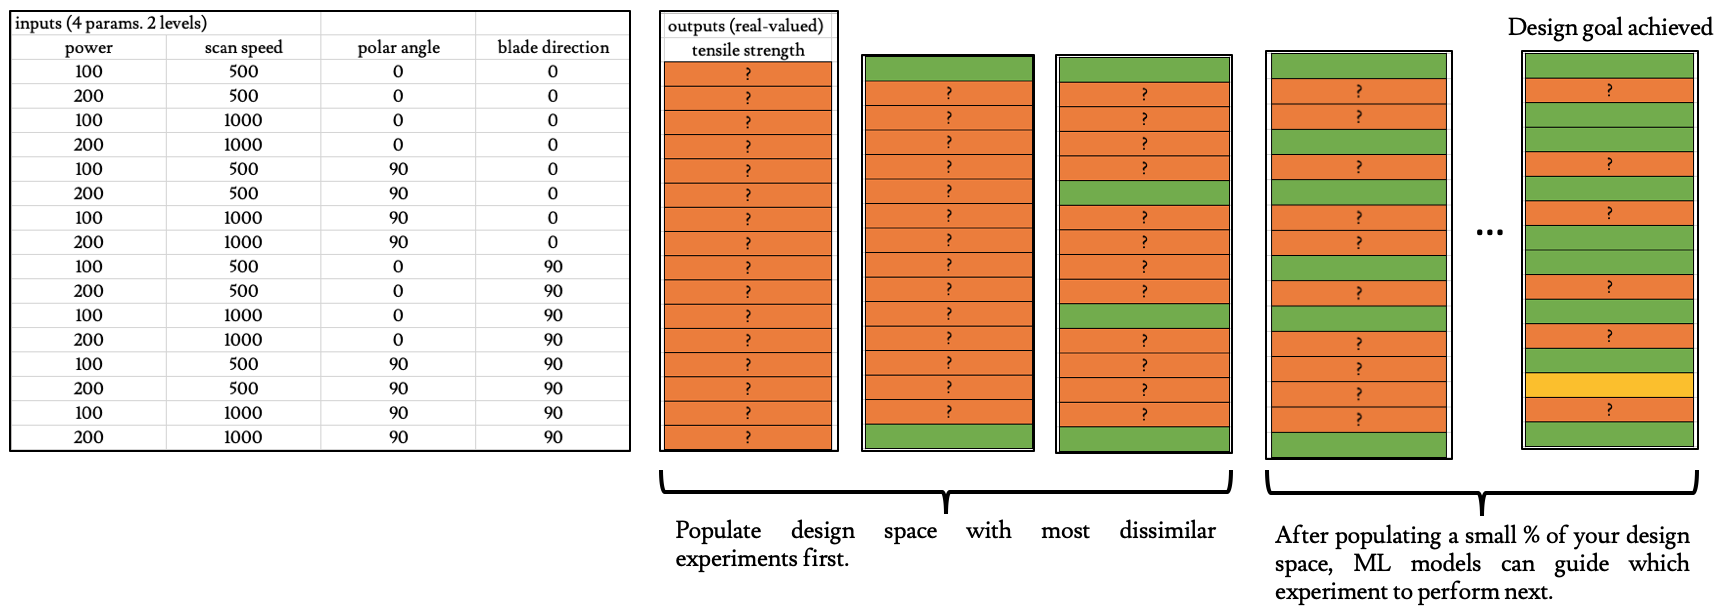
\includegraphics[width=0.9\linewidth]{SectionII/design_example.png}
%  \caption{Illustrating a sequential learning workflow. In this example, there are 16 total possible experiments and
%   4 experiments are performed for initial data collection. To reduce potential bias due subsampling of the input space,
%  the most dissimilar experiments should be performed first. After populating some amount of the design space,
%  machine learning should be used to begin informative data collection until design goal is realized.}
%  \label{fig:SL}
%\end{figure}

%%%

